\section{Tombstone diagram}

A tombstone diagram shows how the interpretation or compilation is done \cite{Tombstone}.
Elements of the diagram have a graphical semantics. 
Interpreters' tombstone diagrams are made with a spade looking figure, with the grip in the top, and the spadestick in the bottom. In the top of the diagram one must put what program is developed, and what language the program is written in. The middle part one must put the interpreter and the machine which is should run on. The interpreter and the language which the program is written in, must be the same, since this is an interpreter. And the spadestick, or the bottom part states the machine which the program should run on.

			\begin{figure}
				\centering
				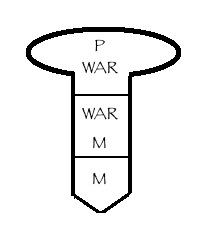
\includegraphics{rapport/3/figures/tombstone}
				\caption{Tombstone Diagram for the WAR language\\ Interpreting a program P expressed in language WAR, using a WAR interpreter runnning on machine M} \label{fig:tombstone}
			\end{figure}
			
In figure \ref{fig:tombstone} one can see that from a program developed in the programming language $WAR$, it will be interpret from the language $WAR$ to the machine $M$ and the interpreter will run on the same machine $M$. By the machine $M$ me mean that is can run on every computer with the .NET framework